\documentclass[11pt]{article}
\usepackage[english]{babel}
\usepackage{minted}
\usepackage{amsmath}
\usepackage{amsthm}
\usepackage{graphicx}
\usepackage{subcaption}
\usepackage{booktabs}
\usepackage{tikz}
\usepackage[left=25mm, top=25mm, bottom=30mm, right=25mm]{geometry}
\usepackage[colorlinks=true, linkcolor=blue, urlcolor=cyan, filecolor=magenta]{hyperref}

\usetikzlibrary{positioning, calc, intersections, shapes.geometric, arrows}
\tikzset{startstop/.style={rectangle, rounded corners, minimum width=3cm, minimum height=1cm,text centered, draw=black, fill=red!30},
         process/.style={rectangle, text width=5.5cm, minimum height=1cm, text centered, draw=black, fill=orange!30},
         io/.style={trapezium, trapezium left angle=70, trapezium right angle=110, text width=3cm, minimum height=1cm, text centered, draw=black, fill=blue!30},
         decision/.style={diamond, aspect=2, text width = 2cm, minimum height=1cm, text centered, draw=black, fill=green!30},
         every arrow/.style={thick,>=stealth}}

\title{COL334\\Assignment 2}
\author{Sayam Sethi}
\date{September 2021}

\begin{document}

\maketitle

\tableofcontents

\section{Preliminaries}
The language used is \texttt{Java} since it offers cross-platform compatibility which is dubious in \texttt{C++} since there is no \textit{standard} library for socket programming. This might lead to incompatibility when running the code on a platform different from the one it has been implemented on. \texttt{Java} is better than \texttt{python} since \texttt{python} is a relatively slower language and networking applications need to be quick to deliver the best performance.

\section{\href{run:./Server.java}{Server.java}}
The logical flow of the server is given as follows:
\begin{center}
    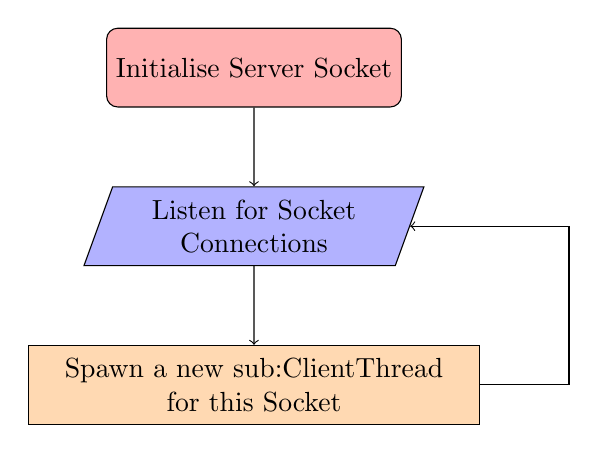
\begin{tikzpicture}[node distance=1cm]
        \node (start)[startstop]{Initialise Server Socket};
        \node (listen)[io, below=of start]{Listen for Socket Connections};
        \draw [->] (start) -- (listen);
        \node (spawn)[process, below=of listen]{Spawn a new \nameref{sub:ClientThread} for this Socket};
        \draw [->] (listen) -- (spawn);
        \draw [->] (spawn) -- ++ (4cm, 0) |- (listen);
    \end{tikzpicture}
\end{center}

\subsection{Client Thread}%
\label{sub:ClientThread}
\begin{center}
    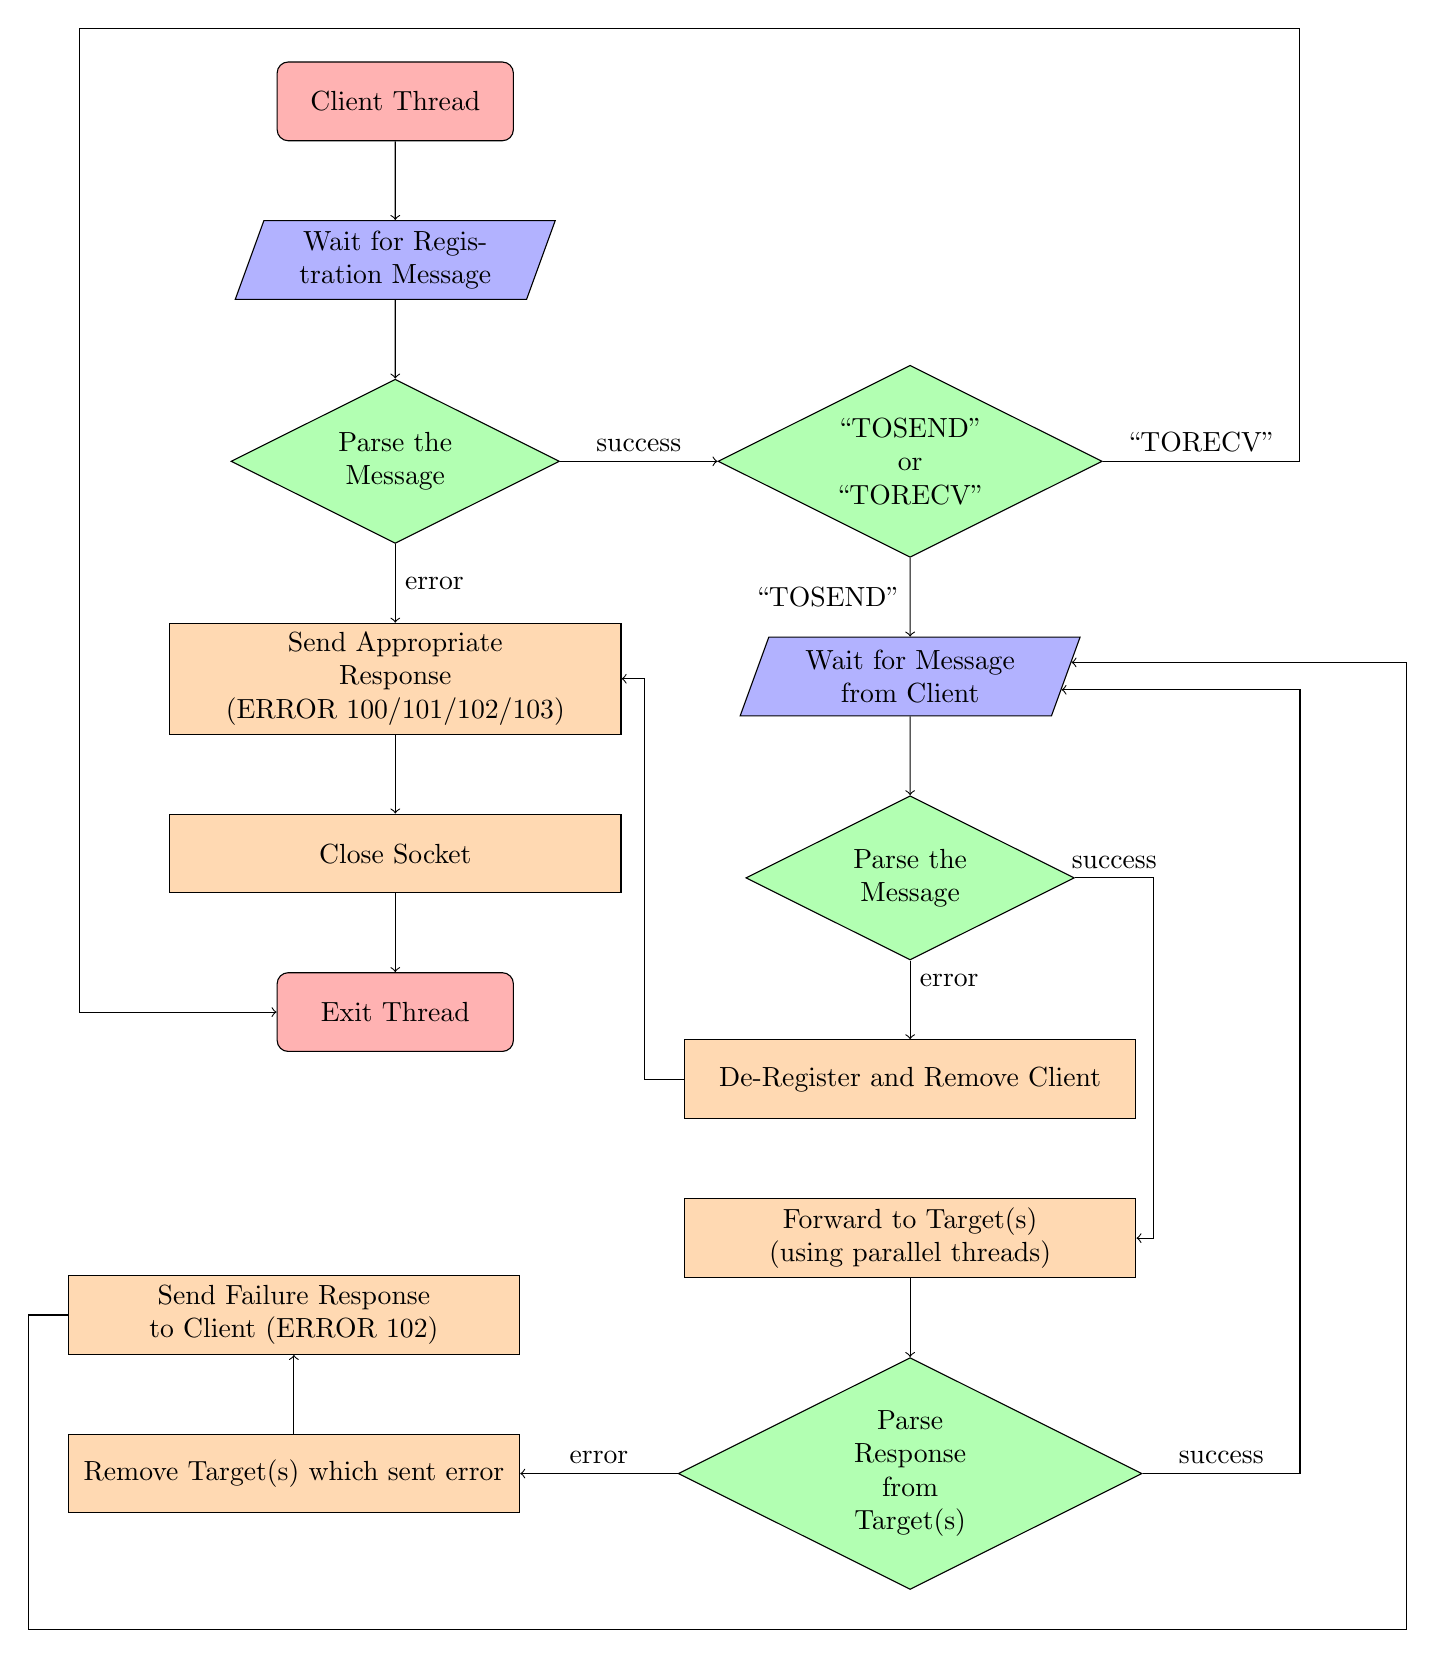
\begin{tikzpicture}[node distance=1cm and 2cm]
        \node (start)[startstop]{Client Thread};
        \node (register)[io, below=of start]{Wait for Registration Message};
        \draw [->] (start) -- (register);
        \node (parsereg)[decision, below=of register]{Parse the Message};
        \draw [->] (register) -- (parsereg);
        \node (err)[process, below=of parsereg]{Send Appropriate\\Response\\(ERROR 100/101/102/103)};
        \node (close)[process, below=of err]{Close Socket};
        \draw [->] (err) -- (close);
        \draw [->] (parsereg) -- node[right, pos=0.5]{error} (err);
        \node (regsuc)[decision, right=of parsereg]{``TOSEND" or ``TORECV"};
        \draw [->] (parsereg) -- node[above, pos=0.5]{success} (regsuc);
        \node (get)[io, below=of regsuc]{Wait for Message from Client};
        \draw [->] (regsuc) -- node[left, pos=0.5]{``TOSEND"} (get);
        \node (parsemsg)[decision, below=of get]{Parse the Message};
        \draw [->] (get) -- (parsemsg);
        \node (remove)[process, below=of parsemsg]{De-Register and Remove Client};
        \draw [->] (parsemsg) -- node[right, pos=0.25]{error} (remove);
        \draw [->] (remove.west) -- ++(-0.5cm, 0) |- (err);
        \node (fwd)[process, below=of remove]{Forward to Target(s) (using parallel threads)};
        \draw [->] (parsemsg.east) -- ++(1cm, 0) node[above, pos=0.5]{success} |- (fwd.east);
        \node (parseres)[decision, below=of fwd]{Parse Response from Target(s)};
        \draw [->] (fwd) -- (parseres);
        \draw [->] (parseres.east) -- ++(2cm, 0) node[above, pos=0.5]{success} |- (get.355);
        \node (fwdremove)[process, left=of parseres]{Remove Target(s) which sent error};
        \draw [->] (parseres) -- node[above, pos=0.5]{error} (fwdremove);
        \node (sendres)[process, above=of fwdremove]{Send Failure Response to Client (ERROR 102)};
        \draw [->] (fwdremove) -- (sendres);
        \draw [->] (sendres.west) -- ++(-0.5cm, 0) |- ++(17.5cm, -4cm) |- (get.365);
        \node (end)[startstop, below=of close]{Exit Thread};
        \draw [->] (close) -- (end);
        \draw [->] (regsuc.east) -- ++(2.5cm, 0) node[above, pos=0.5]{``TORECV"} -- ++(0, 5.5cm) -- ++(-15.5cm, 0) |- (end.west);
    \end{tikzpicture}
\end{center}


\section{\href{run:Client.java}{Client.java}}
The logical flow of the client is given as follows:
\begin{center}
    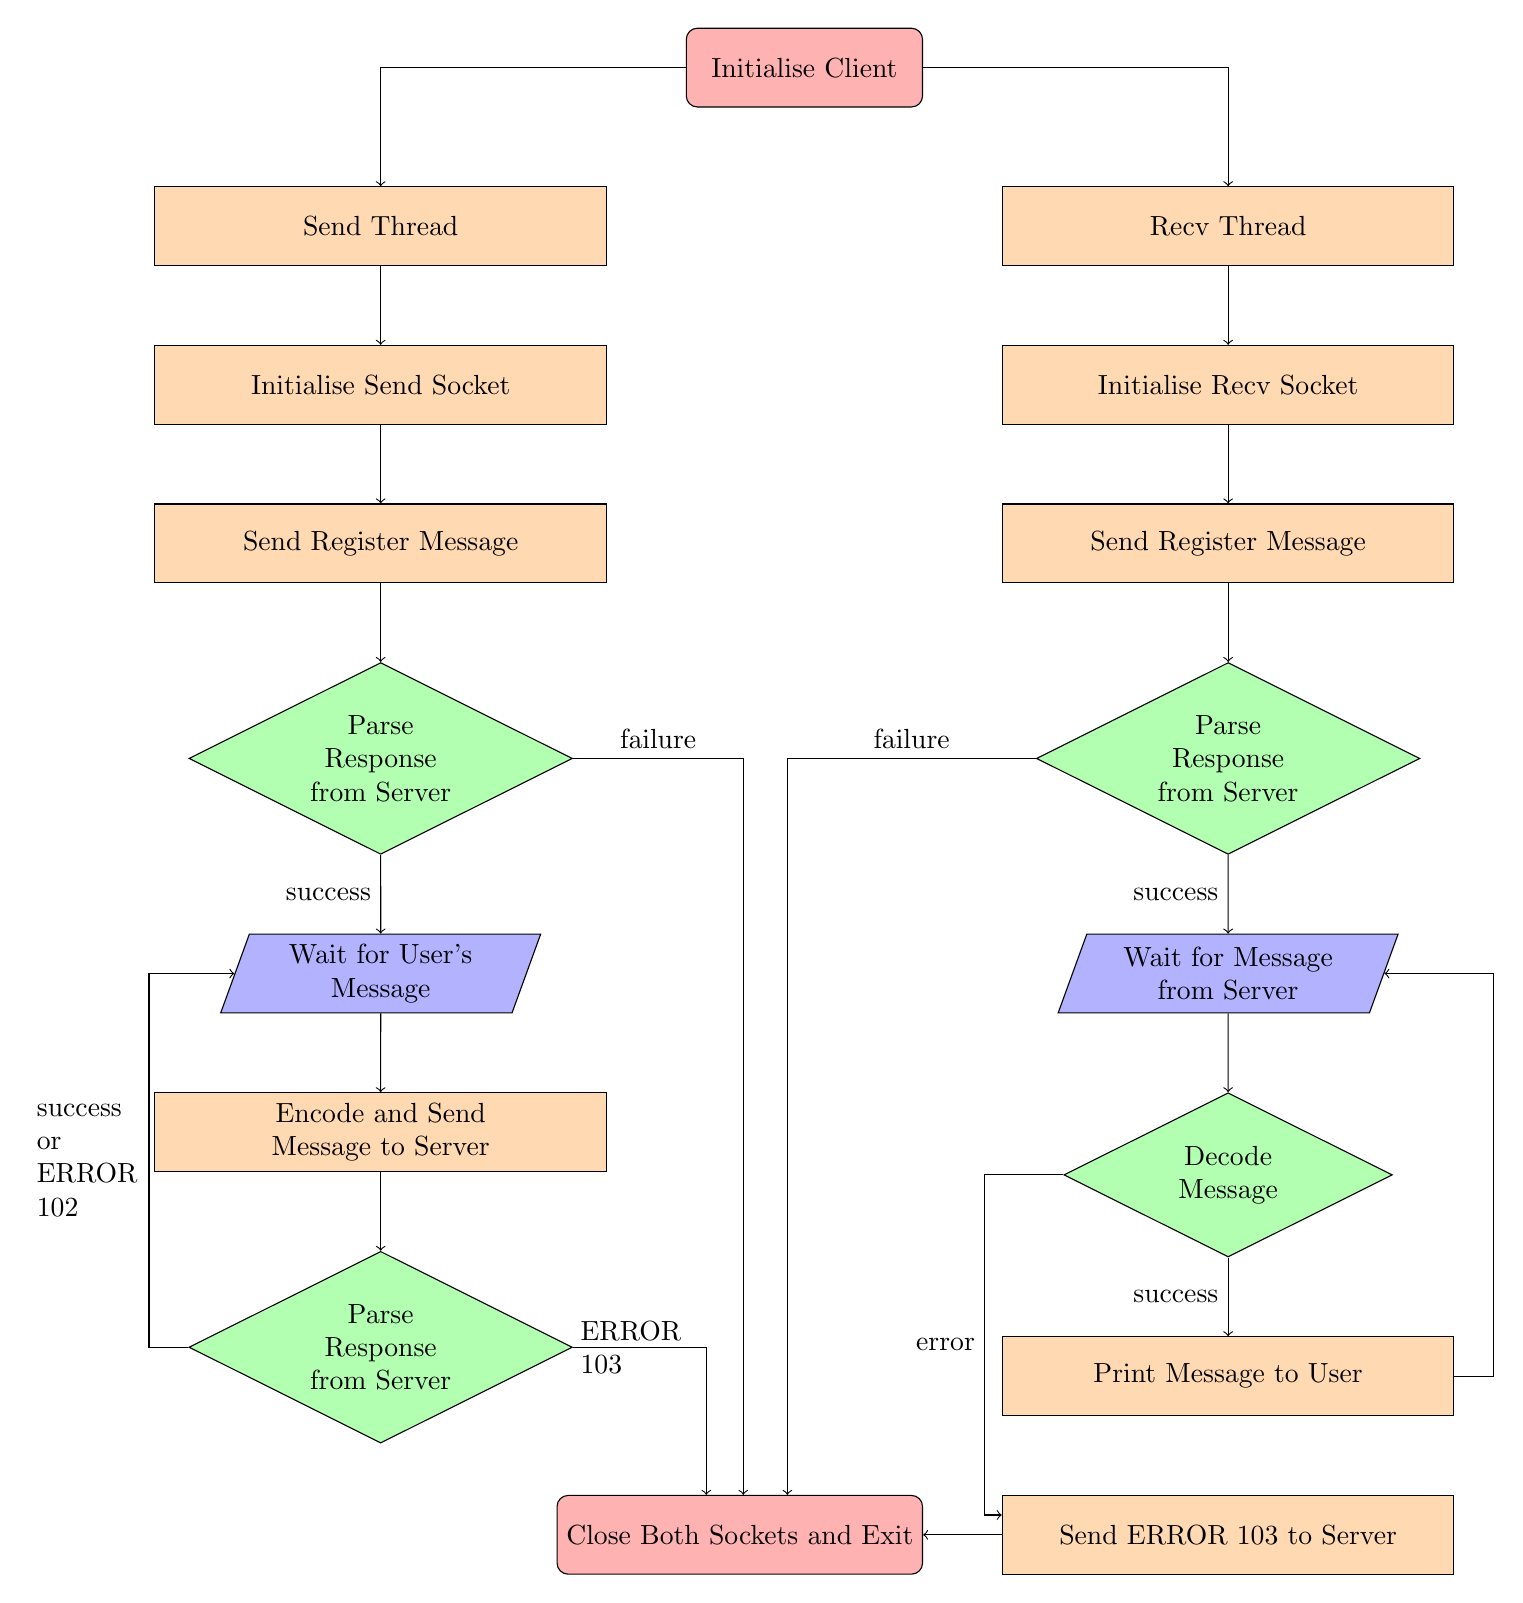
\begin{tikzpicture}
        \node (start)[startstop]{Initialise Client};
        
        \node (sendthread)[process, below left=of start]{Send Thread};
        \draw [->] (start) -| (sendthread);
        \node (sendsocket)[process, below=of sendthread]{Initialise Send Socket};
        \draw [->] (sendthread) -- (sendsocket);
        \node (sendreg)[process, below=of sendsocket]{Send Register Message};
        \draw [->] (sendsocket) -- (sendreg);
        \node (parsesendreg)[decision, below=of sendreg]{Parse Response from Server};
        \draw [->] (sendreg) -- (parsesendreg);
        \node (sendloop)[io, below=of parsesendreg]{Wait for User's Message};
        \draw [->] (parsesendreg) -- node[left, pos=0.5]{success} (sendloop);
        \node (send)[process, below=of sendloop]{Encode and Send Message to Server};
        \draw [->] (sendloop) -- (send);
        \node (parseres)[decision, below=of send]{Parse Response from Server};
        \draw [->] (send) -- (parseres);
        \draw [->] (parseres.west) -- ++(-0.5cm, 0) |- node[left, pos=0.25, text width=1.3cm]{success\\or\\ERROR 102} (sendloop.west);

        \node (recvthread)[process, below right=of start]{Recv Thread};
        \draw [->] (start) -| (recvthread);
        \node (recvsocket)[process, below=of recvthread]{Initialise Recv Socket};
        \draw [->] (recvthread) -- (recvsocket);
        \node (recvreg)[process, below=of recvsocket]{Send Register Message};
        \draw [->] (recvsocket) -- (recvreg);
        \node (parserecvreg)[decision, below=of recvreg]{Parse Response from Server};
        \draw [->] (recvreg) -- (parserecvreg);
        \node (recvloop)[io, below=of parserecvreg]{Wait for Message from Server};
        \draw [->] (parserecvreg) -- node[left, pos=0.5]{success} (recvloop);
        \node (recv)[decision, below=of recvloop]{Decode Message};
        \draw [->] (recvloop) -- (recv);
        \node (print)[process, below=of recv]{Print Message to User};
        \draw [->] (recv) -- node[left, pos=0.5]{success} (print);
        \draw [->] (print.east) -- ++(0.5cm, 0) |- (recvloop.east);
        \node (senderr)[process, below=of print]{Send ERROR 103 to Server};
        \draw [->] (recv.west) -- ++(-1cm, 0) |- node[left, pos=0.25]{error} (senderr.175);

        \node (end)[startstop, below left=of print]{Close Both Sockets and Exit};
        \draw [->] (parsesendreg) -| node[above, pos=0.25]{failure} (end.85);
        \draw [->] (parseres) -| node[pos=0.25, text width=1.5cm]{ERROR 103} (end.130);
        \draw [->] (parserecvreg) -| node[above, pos=0.25]{failure} (end.40);
        \draw [->] (senderr) -- (end);
    \end{tikzpicture}
\end{center}


\end{document}

